\section{Auswertung}
In diesem Kapitel sollen die aufgenommenen Messwerte ausgewertet werden.
Über die Schaltung wurden zudem noch folgende Werte notiert:
\begin{center}
    $L = 16,78 +/- 0,09 \si[]{mH}$,\\
    $C = 2,066 +/- 0,006 \si[]{nF}$,\\
    $R = 67,2 +/- 0,2 \si[]{\Omega}$.\\
\end{center}
\subsection{Berechnung der Abklingdauer}

\label{sec:abklingdauer}
Die aufgenommenen Wertepaare aus Spannung $U(t)$ und $t$ wurden in \autoref{fig:bild1}
aufgetragen und es wurde eine Ausgleichskurve hindurchgelegt. Sie hat die Parameter:
\begin{center}
    
        $a = 3.3568 \pm 0.0669 \Leftrightarrow U_0 = 3.3568 \pm 0.0669 \si{\volt}$ \\
        $b = -1119.1751 \pm 100.4186 \Leftrightarrow \mu = 178.1222 \pm 15.982 \si{\per\second}$ .\\
    
\end{center}  
Der erste Parameter kann hier als Spannung $a=U_0$ interpretiert werden.
Über die Beziehung 
\begin{center}
    $R_{eff} = 4\pi\mu L = -2 L b$
\end{center}


lässt sich der Dämpfungswiderstand $R_{eff}$, mit $L = 16,78 \pm 0,09 \si{mH}$ zu
\begin{center}
    $R_{eff} = 37.6 \pm 3.4 \si{\ohm}$
\end{center}
bestimmen. Damit lässt sich über \autoref{eq:prozentuale} die prozentuale Abweichung des gemessenen
gegenüer des Verbauten Widerstandes $R = 67,2 \pm 0,2  \si{\Omega}$ zu $44\pm 5 \si{\percent}$ bestimmen.
Nun kann auch die Abklingdauer mithilfe des Zusammenhangs
\begin{center}
    $T_{ex} = - \frac{1}{b}$
\end{center}
berechnet werden. Damit folgt sofort:
\begin{center}
    $T_{ex} = 0.00089\pm 0.00008 \si[]{s}$. \\
\end{center}

\begin{figure}
    \centering
    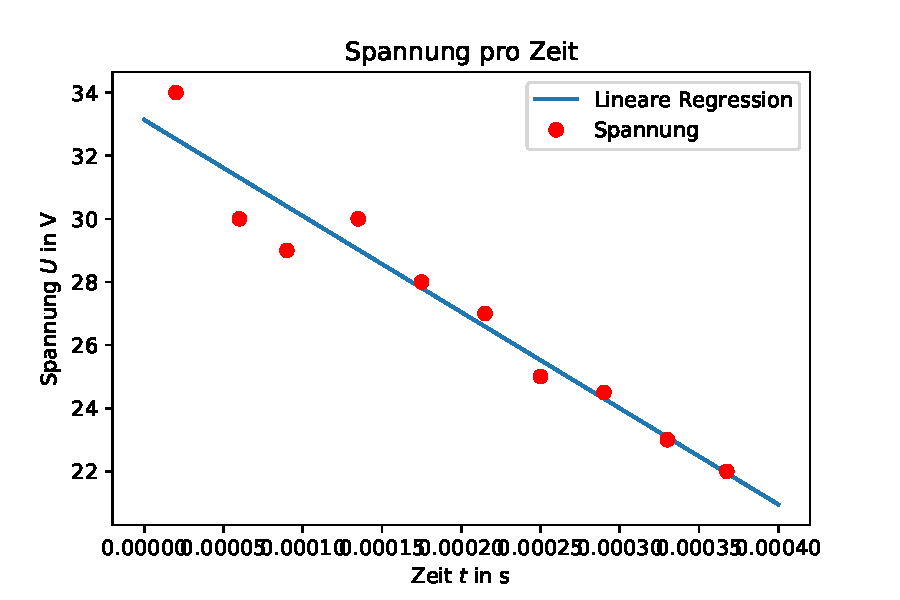
\includegraphics{spannungsverlauf.pdf}
    \caption{Spannungsverlauf in der Zeit}
    \label{fig:bild1}
  \end{figure}

  \subsection{Der Aperiodische Grezfall}
  \label{sec:apg}
  Der Widerstand wurde solange verändert bis der Aperiodische Grenzfall eingetreten ist. Der zu diesem 
  Zeitpunkt eingestellte Widerstand liegt bei:
  \begin{center}
      $R_{ap}=\SI[]{2.91}[]{k\Omega}$.\\
  \end{center}
  Der entsprechende Widerstand lässt sich mit den gegebenen für $L$ und $c$ Werten auch über:
  \begin{center}
      $R_{ap}=2\sqrt{\frac{L}{C}}=5,700+/-0,017\si[]{k\Omega}$
  \end{center}
  bestimmen. Die nach \autoref{sec:prozentuale} berechnete prozentuale Abweichung beträgt 48.94\%.
  Sie lässt sich vorallem dadurch erklären das es schwirig ist exakt den richtigen Widerstand 
  einzustellen da das eintreten des Aperiodischengrenzfalls nur schwer auf dem Osziloskop zu erkennen  ist,
  es handelt sich also um einen Ablesefehler. Erschwerend kommt hinzu das Verschiedene Widerstände von Leitungen
  und Innenwiderstände von Geräten wie dem Oszilloskop und dem Erreger nicht ideal sind.

  \subsection{Resonanzüberhöhung}
  \label{sec:res}
  In \autoref{fig:resonanz} ist die Erregerfrequenz gegen die Spannung halblogaritmisch aufgetragen.
  Die rote Linie zeigt dabei an, wo die Resonanzüberhöhung bzw. die Güte berechnet wurde. In
  \autoref{fig:resonanzzoom} ist nur der Bereich der Resonanzüberhöhung linear dargestellt. Da es keine
  Messwerte gibt weche genau den Wert $\frac{max(U_C)}{U_E*\sqrt{2}}$ mit $U_E=50V$, haben wurde zwischen
  dem jeweils darüber und darunter liegenden Messwert linear interpoliert. Dies führt zu folgenden Ergebnissen:
  \begin{center}
      $\omega_-=\SI[]{25,2245}[]{\kilo\hertz}$,\\
      $\omega_+=\SI[]{26,6224}[]{\kilo\hertz}$.\\
  \end{center}
  Die Güte lässt sich dann einfach über:
  \begin{center}
      $q=\frac{\omega_0}{\omega_+-\omega_-}$,\\
      $\omega_0=\frac{1}{\sqrt{LC}}$,\\
      $\Rightarrow$ $q=\frac{1}{\sqrt{LC}(\omega_+-\omega_-)=121.5\pm 0.4}$
  \end{center} 

  Der thoeretische Wert lässt sich dann über:
  \begin{center}
      $q=\frac{L}{\sqrt{LC}R}$,\\
      $\Rightarrow$  $q=42.41\pm 0.18$\\
  \end{center}
  berechnen. Die über \autoref{eq:prozentuale} berechnete prozentuale Abweichung betraägt dann 186.5\%.
  \begin{figure}
    \centering
    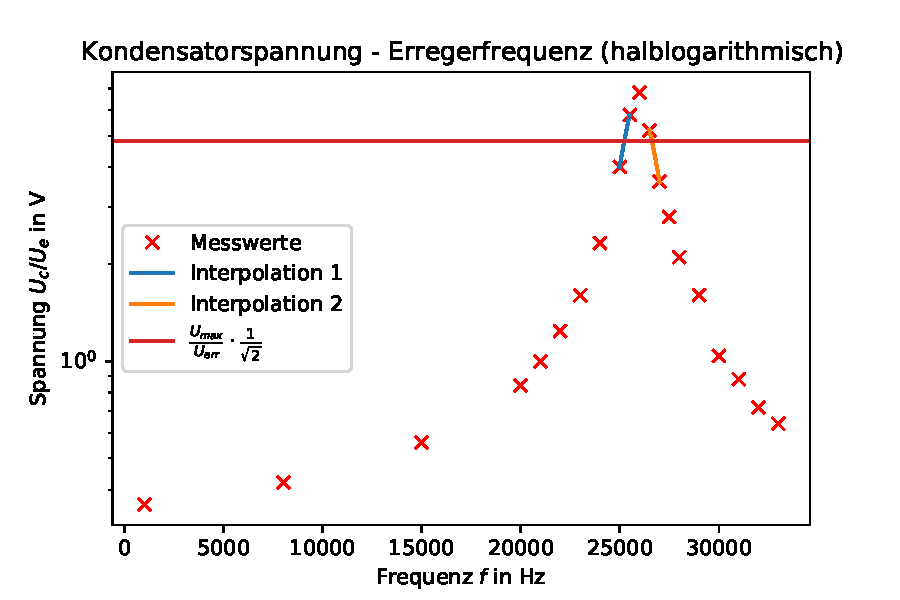
\includegraphics{frequenz.pdf}
    \caption{Spannungsverlauf in Abhängigkeit der Frequenz}
    \label{fig:resonanz}
  \end{figure}

  \begin{figure}
    \centering
    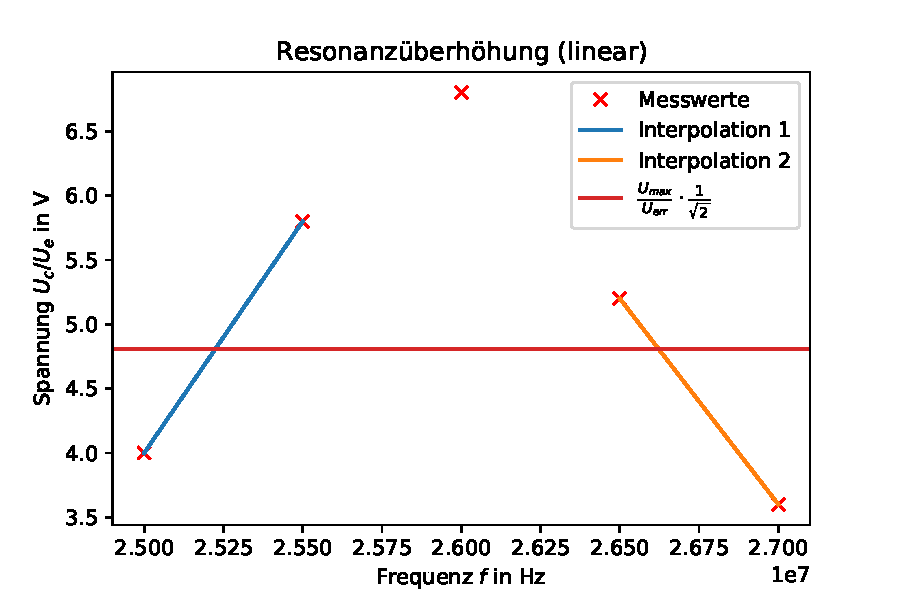
\includegraphics{resonanzuberhohung.pdf}
    \caption{Spannungsverlauf in Abhängigkeit der Frequenz}
    \label{fig:resonanzzoom}
  \end{figure}

\subsection{Phasenverschiebung}
\label{sec:phs}
Aus der als Zeitwerte gemessenen Phasenverschiebung lassen sich über:
\begin{center}
    $\phi=\Delta tf360°$\\
\end{center}
die Phasenverschiebungen in grad berechnen. Sie wurden in \autoref{fig:phasenverschiebung} halblogaritmisch gegen die Frequenz
aufgetragen. In \autoref{fig:phasenverschiebung2} ist der Selbe Sachverhalt nocheinmal linear aufgetragen. Zudem
sind hier noch Graden bei den Winkeln 45°,90° und 135° einetragen. Um die zugehörigen Frequenzen zu finden wurde
wieder linear interpoliert.
\begin{figure}
    \centering
    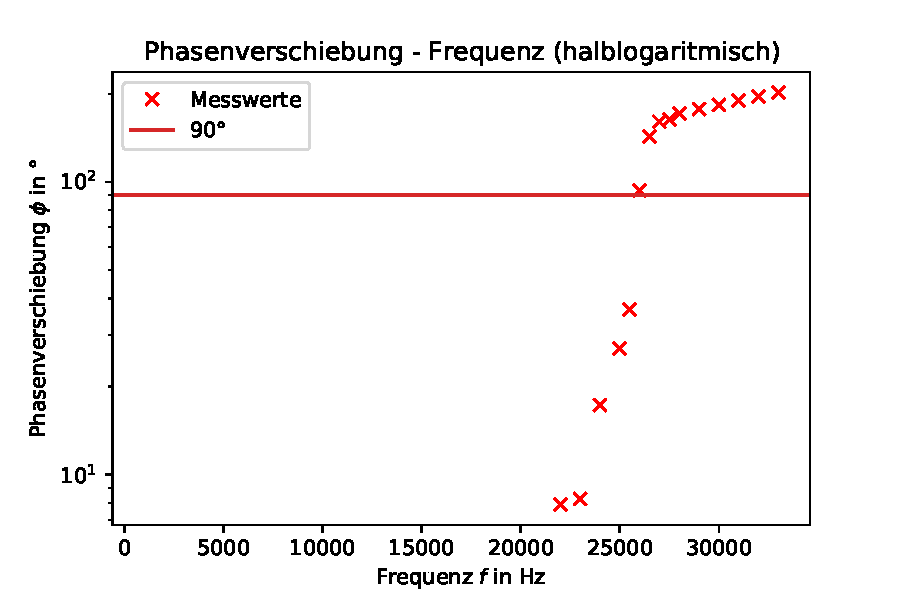
\includegraphics{phasenverschiebung.pdf}
    \caption{Phasenverschiebung in Abhängigkeit der Frequenz.}
    \label{fig:phasenverschiebung}
  \end{figure}
  \begin{figure}
    \centering
    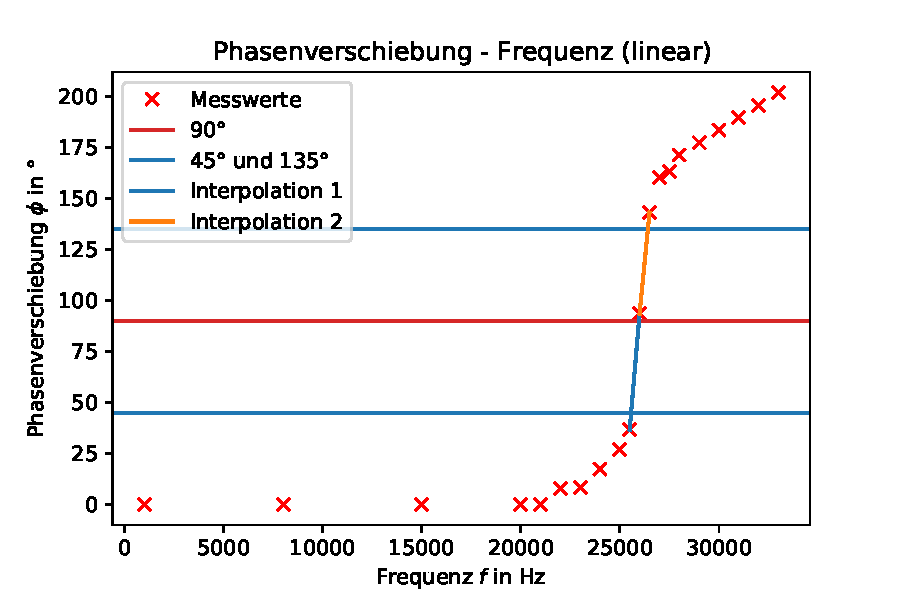
\includegraphics{phasenverschiebunglin.pdf}
    \caption{Phasenverschiebung in Abhängigkeit der Frequenz.}
    \label{fig:phasenverschiebung2}
  \end{figure}
  Die daraus resultierenden Frequenzen lauten:
  \begin{center}
      $45°$$\rightarrow$$\omega_1=\SI[]{25,5728}[]{kHz}$,\\
      $90°$$\rightarrow$$\omega_{res}=\SI[]{25,9684}[]{kHz}$ und\\
      $135°$$\rightarrow$$\omega_2=\SI[]{26,4182}[]{kHz}$.\\
  \end{center}
  Die theoretischen pendants lassen sich über die nachstehenden Gleichungen bestimmen.
  \begin{center}
      $\omega_{1,2}=\pm \frac{R}{2L}+\sqrt{\frac{R^2}{4L^2}+\frac{1}{LC}}$,\\
      $\omega_{res}=\sqrt{\frac{1}{LC}-\frac{R^2}{2L^2}}$
  \end{center}
Damit folgt dann sofort:
\begin{center}
    $45°$$\rightarrow$$\omega_1=(2.774\pm 0.011) \times 10^5\si[]{Hz}$,\\
    $90°$$\rightarrow$$\omega_{res}=(1.0398\pm 0.0027)\times 10^5\si[]{kHz}$ und\\
    $135°$$\rightarrow$$\omega_2=(1.175\pm 0.004)\times 10^5\si[]{kHz}$.\\
  \end{center}
\end{center}
 
Die nach \autoref{eq:prozentuale} berechneten relativen Abweichungen betragen für $\omega_1$ 90.78\%, für 
$\omega_2$ 77,9\% und für $\omega_{res}$ 74,59\%.














 

